\section{模块 3 · 步骤 2 上篇：把点云变成``图上的楼块''}

从这个模块起讲具体算法。步骤 2（单体分割）在代码里是一条流水线
（\texttt{instance\_segmentation\_v2.py}），本模块讲前半段：
\textbf{栅格化 $\to$ 连通域}，以及一个用真实失败换来的设计决定（\textbf{不做闭运算}）。
后半段（拆粘连、防过分割）在模块 4。

\subsection{第一刀：把三维点云``拍扁''成二维格子图（栅格化）}

\textbf{栅格化（rasterization）}就是把连续空间切成规则小方格（想象一张方格纸铺在地图上），
再统计每个格子里落了什么。我们在俯视视角下铺一张\textbf{边长 0.5 米}的方格纸，
把 863 万个建筑点按 $(x,y)$ 坐标投进格子里。

为什么可以放心``拍扁''（丢掉俯视重叠信息）？因为在住宅区里，
两栋不同的楼在俯视图上不会上下重叠——``按栋分开''本质上是个二维问题。
但注意：我们并没有真的丢掉高度。每个格子除了记``落了几个点''，
还记下了\textbf{格内最高点的高程 $z_{\max}$}——这张``高度图''在模块 4 的分水岭里是主角。

接着定义哪些格子``算数''：

\begin{center}
\fbox{\parbox{0.9\textwidth}{\centering
\textbf{占据规则}：一个格子里落入 $\geq 2$ 个建筑点，才算``被建筑占据''。
}}
\end{center}

为什么是 $\geq 2$ 而不是 $\geq 1$？这是\textbf{第一道防线}：RandLA-Net 偶尔会把一两个零星的
树点、车点错标成``建筑''。若 1 个点就算占据，一串零星错点就能在两栋楼之间搭出一条
``一点宽的桥''，把两栋楼连起来。要求每格至少 2 点，孤立错点自动失效。
说它是``第一道''防线是有分寸的：它只压低搭桥的概率，不能保证根除
（理论上两个错点挤进同一格仍能过关）——彻底的保障靠的是它与后续机制的叠加
（模块 4 的分水岭还会按高度把粘连切开）。代价方面：全区平均密度约 30 点/m\textsuperscript{2}
（0.5 m 格子平均 7--8 个点），完整屋面的格子远超 2 点的门槛；
真正可能受损的是屋顶边缘和被树遮挡处的稀疏格子——这些格子里的点先被放下，
模块 4 结尾有专门的``孤儿点回挂''机制把它们捡回来。

\begin{figure}[H]
\centering
\begin{tikzpicture}[scale=0.62]
% 网格
\draw[step=1, gray!40, thin] (0,0) grid (10,5);
% 房子1的点（左）
\foreach \p in {(0.3,1.2),(0.7,1.5),(1.2,1.3),(1.5,1.8),(0.5,2.3),(1.3,2.6),(1.7,2.2),(2.3,1.4),(2.6,1.7),(2.2,2.5),(2.7,2.3),(0.4,3.3),(1.4,3.5),(2.5,3.4),(1.9,3.2),(0.8,2.7),(2.8,3.7),(1.1,1.9),(2.1,1.9),(0.6,3.6)}
  \fill[blue!70] \p circle (2.2pt);
% 房子2的点（右）
\foreach \p in {(6.4,1.3),(6.8,1.6),(7.3,1.4),(7.6,1.9),(6.6,2.4),(7.4,2.7),(7.8,2.3),(8.4,1.5),(8.7,1.8),(8.3,2.6),(8.8,2.4),(6.5,3.4),(6.2,3.7),(7.5,3.6),(7.8,3.3),(8.6,3.5),(8.0,3.3),(6.9,2.8),(7.2,2.0),(8.2,2.0),(6.3,2.9),(8.9,3.1)}
  \fill[blue!70] \p circle (2.2pt);
% 中间一个零星错点
\fill[red!80] (4.6,2.4) circle (2.6pt);
\node[red!80, font=\scriptsize] at (4.6,3.0) {零星错点（1 点）};
% 占据格着色
\begin{scope}[on background layer]
\foreach \c in {(0,1),(1,1),(2,1),(0,2),(1,2),(2,2),(0,3),(1,3),(2,3)}
  \fill[blue!15] \c rectangle +(1,1);
\foreach \c in {(6,1),(7,1),(8,1),(6,2),(7,2),(8,2),(6,3),(7,3),(8,3)}
  \fill[blue!15] \c rectangle +(1,1);
\end{scope}
\node[font=\small] at (1.5,-0.6) {楼 A：格内点多 $\Rightarrow$ 占据};
\node[font=\small] at (7.5,-0.6) {楼 B：占据};
\node[font=\small, red!70!black] at (4.5,0.4) {仅 1 点的格子不算占据};
\end{tikzpicture}
\caption{栅格化与占据规则：点（蓝）投进 0.5 m 格子；$\geq2$ 点的格子（浅蓝）构成``占据图''；
孤立错点（红）无法形成占据格，从源头掐断``一点桥''。}
\label{fig:raster}
\end{figure}

这一步结束，863 万个建筑点的问题被压缩成一张黑白图像：黑格 = 有建筑，白格 = 没有。
后面的所有操作都在这张图上做，这正是模块 2 说的 Song \& Jung 路线的精髓
——\textbf{图像化之后，几十年积累的图像处理工具全部可用}。

\subsection{第二刀：连通域标记——``挨着的格子算同一块''}

\textbf{连通域（connected component）}是图像处理最基础的概念：
在黑白图上，把互相挨着的黑格归成一``块''，每块发一个编号。
``挨着''有两种定义：\textbf{4-连通}只认上下左右四个邻居；
\textbf{8-连通}把四个斜对角也算邻居。我们用 8-连通
（屋顶边缘呈锯齿状时,斜向相邻的格子理应属于同一栋楼）。

\begin{figure}[H]
\centering
\begin{tikzpicture}[scale=0.55]
\begin{scope}
\draw[step=1, gray!50] (0,0) grid (3,3);
\fill[blue!25] (1,1) rectangle (2,2);
\foreach \c in {(1,0),(0,1),(2,1),(1,2)} \fill[blue!60] \c rectangle +(1,1);
\node[font=\small, align=center] at (1.5,-1.0) {4-连通：\\ 只认上下左右};
\end{scope}
\begin{scope}[xshift=13cm]
\draw[step=1, gray!50] (0,0) grid (3,3);
\fill[blue!25] (1,1) rectangle (2,2);
\foreach \c in {(1,0),(0,1),(2,1),(1,2),(0,0),(2,0),(0,2),(2,2)} \fill[blue!60] \c rectangle +(1,1);
\node[font=\small, align=center] at (1.5,-1.0) {8-连通：斜角也算邻居\\ （本项目采用）};
\end{scope}
\end{tikzpicture}
\caption{中心格（浅蓝）的``邻居''（深蓝）在两种连通定义下的范围。}
\label{fig:conn}
\end{figure}

对占据图做一次 8-连通标记，就得到了\textbf{初步的``楼块''}：
绝大多数块确实恰好是一栋楼。但有两类问题留给后面处理：
（a）少数块里粘着两栋以上的楼（模块 4 用分水岭拆）；
（b）屋顶内部有``洞''——烟囱、天窗、被树冠遮挡扫不到的区域，
会让一栋楼的图斑里缺一块。洞本身不影响分块，但会影响后续面积统计和形状判断，需要补上。
\textbf{怎么补洞，恰恰是 v1 版本栽跟头的地方}——这是本模块最重要的一段。

\subsection{v1 的真实教训:``闭运算''为什么会把一排楼焊成一条}

先补两个图像处理的基础词。\textbf{形态学操作（morphological operations）}
是对黑白图的一类``修形''操作，最基本的两个：
\textbf{膨胀（dilation）}——所有黑色区域向外长一圈；
\textbf{腐蚀（erosion）}——反过来，所有黑色区域向内削一圈。
``一圈''有多厚由\textbf{结构元}决定：结构元就是一个小模板，
规定每次向周围扩（或削）多远——比如 $3\times3$ 结构元 = ``中心格加它周围一圈''，
膨胀一次就让区域向四面八方各长出 1 个格子。
\textbf{闭运算（closing）= 先膨胀、再腐蚀}：直觉效果是``小缝被填上、小洞被补齐，
而整体轮廓大致回到原位''——听起来正是``补洞''的完美工具，
也是这类工作流的常见默认选择。

问题出在``\textbf{填小缝}''上。膨胀是不分青红皂白向\textbf{所有}方向长的：
屋顶内部的洞会被填上（好事），但\textbf{两栋楼之间的窄缝也会被填上}（灾难）。
这里小白最该问的问题是：\textbf{腐蚀不是膨胀的反向操作吗，为什么救不回来？}
因为膨胀之后两块已经连成\textbf{一个}实心整体，``缝''作为边界已经不存在了；
腐蚀只会沿着\textbf{当前整体的外边界}向内削，它不记得哪些格子是刚长出来的，
更不知道原来缝在哪里——外圈被削回原位，\textbf{楼与楼之间新长出的``桥''却留在原地}。
在这张占据图上，缝的信息就此\textbf{丢失}，后面的连通域标记自然把两栋楼当成一块。

\begin{figure}[H]
\centering
\begin{tikzpicture}[scale=0.5]
% 原图
\begin{scope}
\fill[blue!60] (0,0) rectangle (3,3);
\fill[blue!60] (5,0) rectangle (8,3);
\fill[white] (1.2,1.2) rectangle (1.8,1.8);
\node[font=\small] at (4,-0.8) {原图：两栋楼，缝 2 m，左楼有洞};
\draw[<->, red!70!black, thick] (3,1.5) -- (5,1.5) node[midway, above, font=\scriptsize]{窄缝};
\end{scope}
% 膨胀
\begin{scope}[xshift=10.5cm]
\fill[blue!25] (-0.5,-0.5) rectangle (8.5,3.5);
\fill[blue!60] (0,0) rectangle (8,3);
\node[font=\small] at (4,-1.3) {膨胀后：洞填上了，\textbf{缝也没了}};
\end{scope}
% 腐蚀
\begin{scope}[yshift=-6.2cm, xshift=5cm]
\fill[blue!60] (0,0) rectangle (8,3);
\node[font=\small] at (4,-0.8) {再腐蚀（=完成闭运算）：外圈缩回去，};
\node[font=\small] at (4,-1.6) {但两楼之间的桥留下了 $\Rightarrow$ 永久焊接（欠分割）};
\end{scope}
\end{tikzpicture}
\caption{闭运算的桥接机理：膨胀无差别外扩，把楼间窄缝一并填死；腐蚀救不回来。}
\label{fig:closing}
\end{figure}

这不是理论风险，是 v1 版本的\textbf{实测事故}。v1 的处理顺序是
``整张占据图先做闭运算，再做连通域标记''，格子 1 米、结构元 $3\times3$：
膨胀一次，每块向四面八方各长 1 格（= 1 米），\textbf{相邻两块相向各长 1 米，
合计能吃掉约 2 米的空隙}。而本区独栋住宅的侧院间隙是 1.5--2.5 米
——其中 2 米及以下的窄缝会被直接糊住；再算上屋檐向外挑出、点落格时的取整，
实际留在图上的缝比侧院本身更窄，遭殃的范围比理论值更大。
后果在实测中显形：整排相邻的独栋被串成一个实例。这个错误是\textbf{用户在
CloudCompare 里逐栋抽查时亲手抓到的}：点开一个具体位置
（我们在代码里记下了这个检查点坐标），发现十几栋房子共用同一个实例编号。

\begin{warnbox}[：v1 $\to$ v2 的两处修复]
\begin{enumerate}
\item \textbf{彻底去掉闭运算，并调换顺序}。v2 改为``\textbf{先}连通域标记，
      \textbf{再}对每块\textbf{单独}补洞''；补洞改用``填洞函数''
      （\texttt{binary\_fill\_holes}）：它只填\textbf{被黑色区域完全包围}的白色区域
      （真正的``洞''），对朝外开口的缝隙无能为力——这正是我们要的：
      \textbf{洞照补，桥绝不搭}；又因为逐块单独执行，两块之间永远不发生相互作用。
\item \textbf{格子从 1 米加密到 0.5 米}。格子越细，窄缝在图上占的格子越多，
      被意外糊住的风险越小，边界也更精细。
\end{enumerate}
修复后在同一检查点复查：原来串成一条的十几栋楼被正确分成独立实例
（图~\ref{fig:checkpoint} 是 v2 的复查图；做 PPT 时可以再从 v1 的存档输出
截取同一窗口，拼成前后对照）。
\end{warnbox}

\begin{figure}[H]
\centering
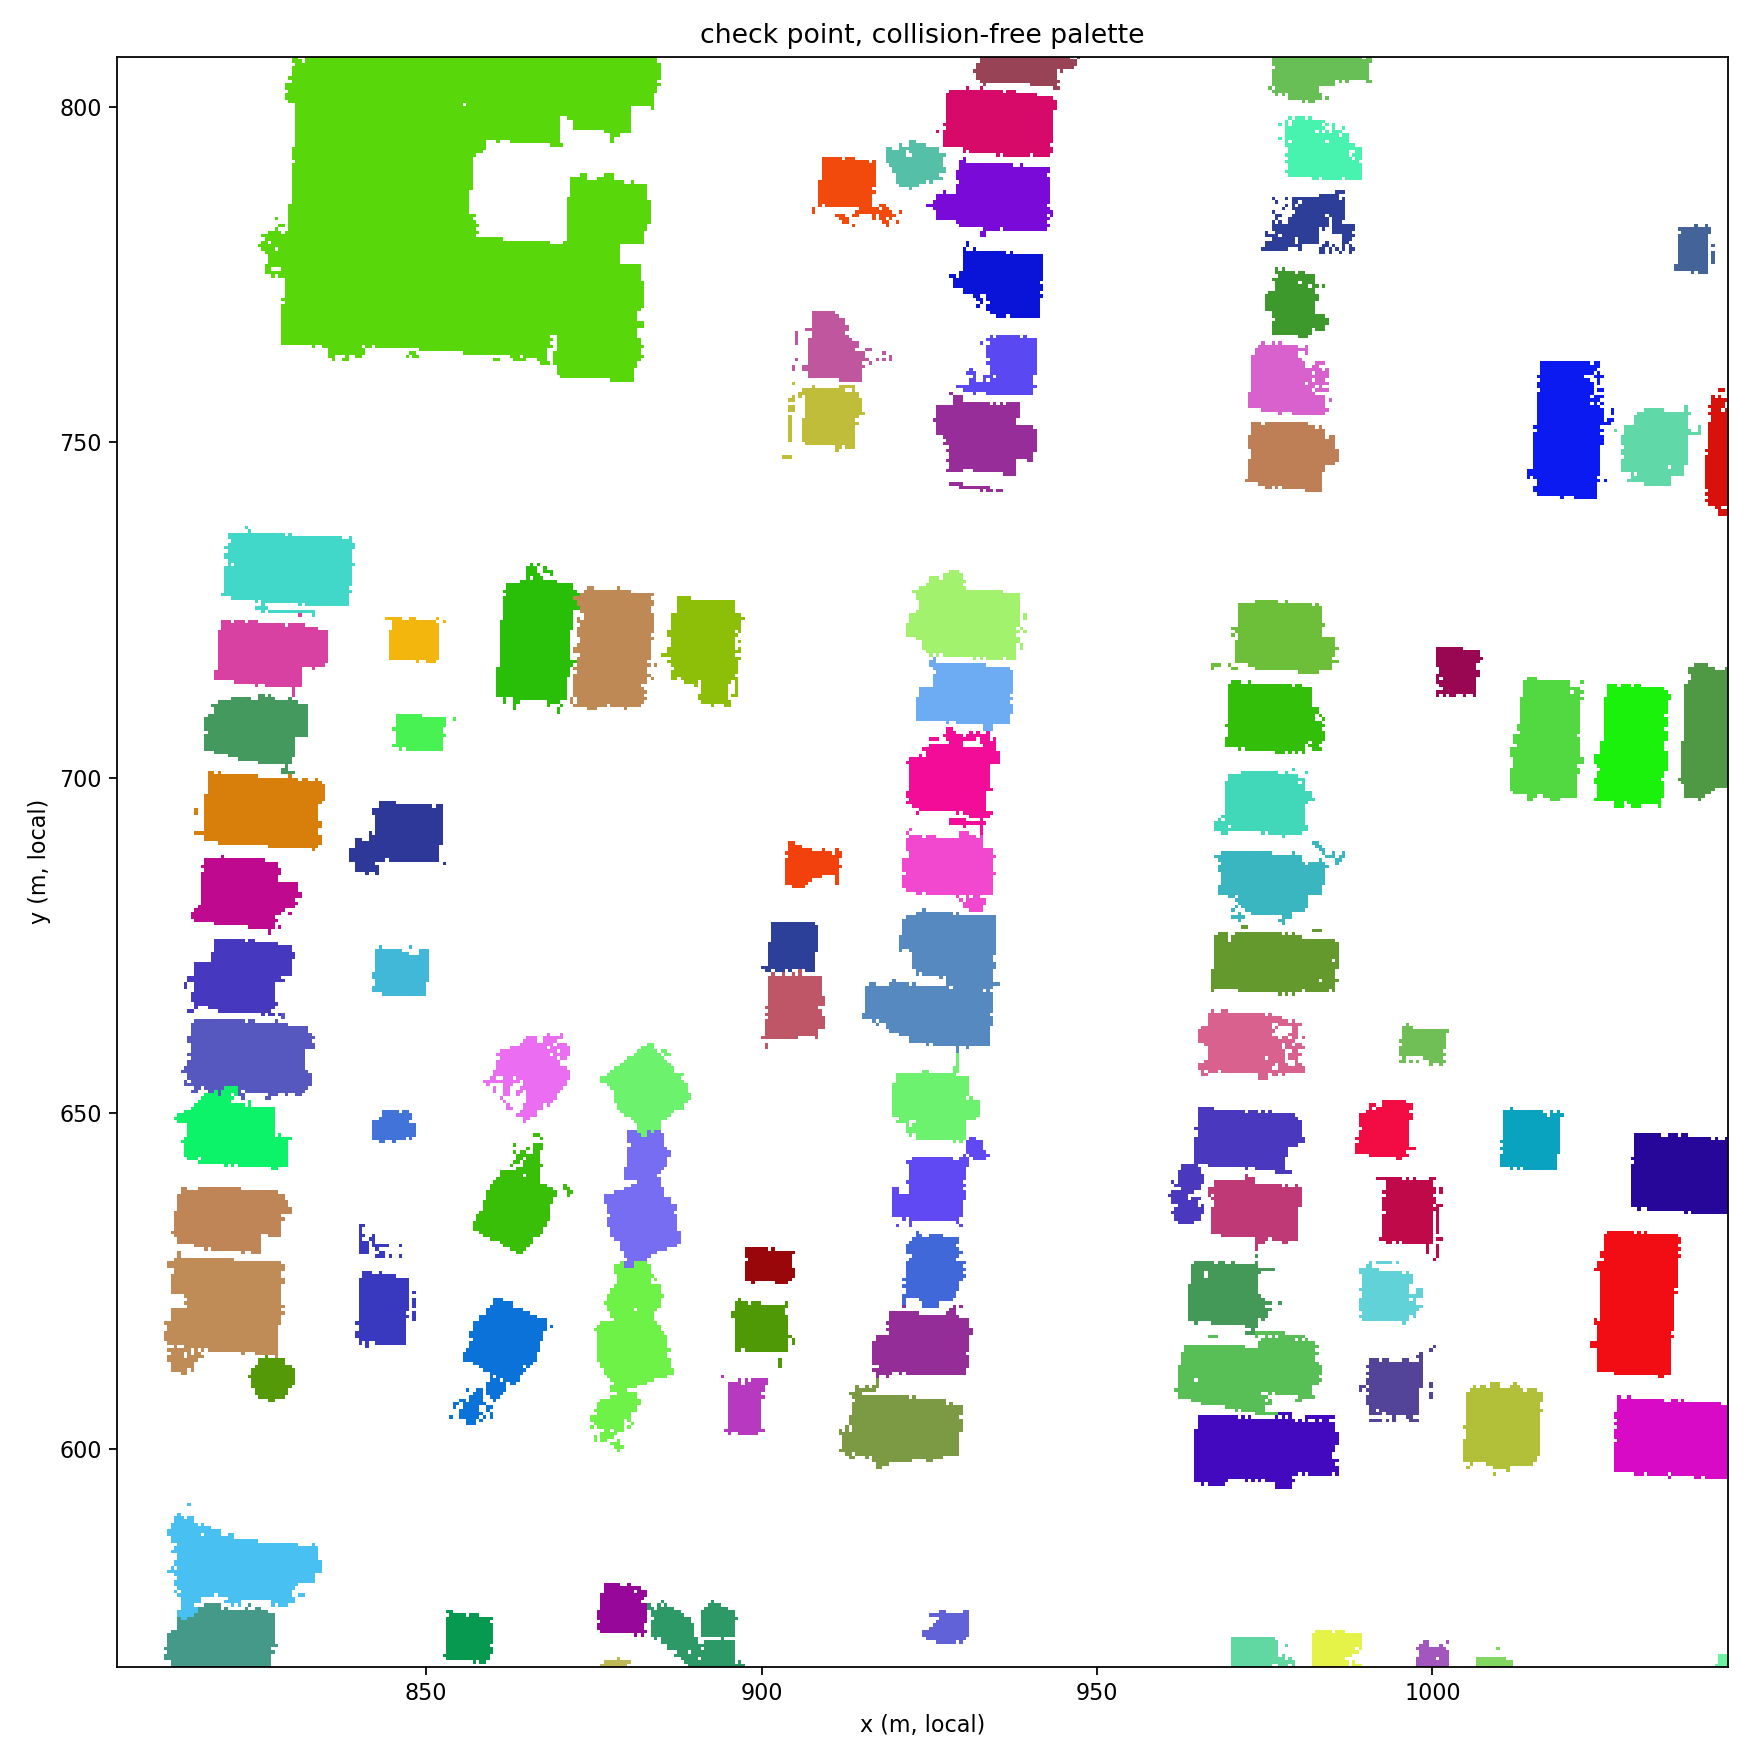
\includegraphics[width=0.72\textwidth]{figs/qa_checkpoint_rgb.png}
\caption{v2 在用户检查点的复查图（每个实例随机配色，颜色仅用于区分相邻实例，
颜色本身不代表对错）：此处正是 v1 把一排独栋串成同一实例的位置，
v2 中这排楼已各自成块、编号互不相同。}
\label{fig:checkpoint}
\end{figure}

\begin{plainbox}[：模块 3 小结]
\begin{itemize}
\item 把 863 万建筑点投进 0.5 m 方格纸，每格 $\geq2$ 点才算占据（掐死``一点桥''），
      同时每格记下最高点高程 $z_{\max}$ 备用。
\item 8-连通标记得到初步楼块；补洞改为逐块``只填包围洞''，
      \textbf{坚决不用闭运算}——v1 的欠分割事故证明：闭运算约 2 m 的桥接能力
      正落在本区 1.5--2.5 m 的侧院区间内，实测把成排独栋焊成了一个实例。
\item 遗留问题：仍有一批块粘着多栋楼。下一模块：怎么发现它们、怎么拆开。
\end{itemize}
\end{plainbox}
